\id{ҒТАМР 65.53.30}{}

\begin{articleheader}
\sectionwithauthors{Л.С.Сыздыкова, К.М.Абдиева, Г.Д. Шамбулова, С.Т. Азимова, Г.Н. Жаксылыкова, А.М. Таева}{КӨКӨНІС ДӘМТАҒАМ КОНСЕРВІЛЕРІН ӨНДІРУДЕ БЕЛСЕНДІ ПЕКТИНГЕ БАЙ ӨСІМДІК ЭКСТРАКТЫСЫН ҚОЛДАНУ}

{\bfseries
Л.С. Сыздыкова\alink{https://orcid.org/0000-0002-8953-6332},
К.М. Абдиева\alink{https://orcid.org/0000-0003-0111-6737}\textsuperscript{\envelope },
Г.Д. Шамбулова\alink{https://orcid.org/0000-0001-6257-1317},
С.Т. Азимова\alink{https://orcid.org/0000-0002-8992-8889},
Г.Н. Жаксылыкова\alink{https://orcid.org/0000-0003-0563-4304},
А.М. Таева\alink{https://orcid.org/0000-0001-6663-4282}
}
\end{articleheader}

\begin{affiliation}
Алматы технологиялық университеті, Алматы қ., Қазақстан

\raggedright \textsuperscript{\envelope }Корреспондент-автор: k.abdiyeva08@gmail.com
\end{affiliation}

Ғылыми жұмыстың мақсаты күнделікті тұтынуға арналған тағам өнімдерінің
ассортиментін табиғи антиоксиданттармен және биологиялық белсенді
заттармен байыту арқылы кеңейту, сондай-ақ отандық өсімдік шикізаты
негізінде дайындалған тағам өнімдерінің тағамдық және биологиялық
құндылығын арттыру мәселелерін шешуге бағытталған. Бұл зерттеу жұмысы
көкөніс дәмтағам консервілерінің ассортиментін кеңейту мақсатында томат
тұздығымен құйылған фаршпен және кесіліп қуырылған көкөністерден
жасалған дәмтағам консервілеріндегі көкөніс фаршының құрамына кіретін
күріштің орнын қарақұмық және булгур жармаларымен алмастыру және
өсімдіктерден алынған белсенді пектинге бай экстрактыларды қолдануға
арналған.

Белсенді пектинге бай экстракттар алу үшін өсімдік шикізатынан зерттеу
үшін алма, асқабақ және кәдіш алынып олардың сапалық көрсеткіштері, яғни
шикізаттағы жалпы пектиндік заттар, еритін пектин мөлшері және
антиоксиданттық белсенділігі анықталды.

Ғылыми жұмыс барысында көкөніс дәмтағам консервілерін дайындауда фарштың
құрамына қосылатын күріштің орнын булгур және қарақұмық жармаларымен
алмастыру арқылы дәмтағам консервілерінің жаңа рецептуралары алынды.
Сондай-ақ жаңа жарма қосылған көкөніс дәмтағам консервілерінің
рецептураларын құрастыруда пектиндік және антиоксиданттық қасиеттері
жағынан \\ерекшеленетін алма және асқабақ пектиндерінің экстрактылары
қолданылды.

{\bfseries Түйін сөздер:} көкөніс дәмтағам консервілері, булгур және
қарақұмық жармалары, пектин заттар мөлшері, рецептура

\begin{articleheader}
{\bfseries ИСПОЛЬЗОВАНИЕ РАСТИТЕЛЬНЫХ ЭКСТРАКТОВ, БОГАТЫХ АКТИВНЫМ ПЕКТИНОМ, В ПРОИЗВОДСТВЕ ОВОЩНЫХ ЗАКУСОЧНЫХ КОНСЕРВОВ}

{\bfseries
Л.С. Сыздыкова,
К.М. Абдиева\textsuperscript{\envelope },
Г.Д. Шамбулова,
С.Т. Азимова,
Г.Н. Жаксылыкова,
А.М. Таева
}
\end{articleheader}

\begin{affiliation}
Алматинский технологический университет, Алматы, Казахстан,

e-mail: k.abdiyeva08@gmail.com
\end{affiliation}

Цель научной работы - расширение ассортимента пищевых продуктов
повседневного потребления за счёт обогащения их природными
антиоксидантами и биологически активными веществами, а также решение
задач по повышению пищевой и биологической ценности продуктов питания,
приготовленных на основе отечественного растительного сырья. Данное
исследование направлено на расширение ассортимента овощных
гастрономических консервов за счёт замены риса, входящего в состав
овощного фарша, на гречневую и булгур крупы, а также использования
экстрактов, богатых активным пектином, полученных из растений, при
производстве гастрономических консервов из жареных нарезанных овощей с
томатным соусом и фаршем.

Для получения экстрактов, богатых активным пектином, в качестве
растительного сырья для исследования были выбраны яблоки, тыква и
кабачки, и определены их качественные показатели, такие как общее
содержание пектиновых веществ, количество растворимого пектина и
антиоксидантная активность.

В ходе научной работы были разработаны новые рецептуры гастрономических
овощных консервов путём замены риса в составе фарша на булгур и
гречневую крупу. Также при разработке рецептур овощных гастрономических
консервов с добавлением новых видов круп использовались экстракты
яблочного и тыквенного пектина, отличающиеся своими пектиновыми и
антиоксидантными свойствами.

{\bfseries Ключевые слова:} овощные закусочные консервы, булгурная и
гречневая крупа, содержание пектиновых веществ, рецептура

\begin{articleheader}
{\bfseries THE USE OF PLANT EXTRACTS RICH IN ACTIVE PECTIN IN THE PRODUCTION OF VEGETABLE APPETIZER PRESERVES}

{\bfseries
L.S. Syzdykova,
K.M. Abdiyeva\textsuperscript{\envelope },
G.D. Shаmbulоvа,
S.T. Aаzimova,
G.N. Zhакsylykova,
A.M. Tayeva
}
\end{articleheader}

\begin{affiliation}
Almaty Technological University, Almaty, Kazakhstan,

e-mail: k.abdiyeva08@gmail.com
\end{affiliation}

The aim of the research is to expand the range of food products intended
for daily consumption by enriching them with natural antioxidants and
biologically active substances, as well as to address the issues of
improving the nutritional and biological value of food products made
from domestic plant raw materials. This study is focused on expanding
the assortment of vegetable culinary preserves by replacing rice, which
is part of the vegetable stuffing, with buckwheat and bulgur groats, and
by using plant-derived extracts rich in active pectin for the production
of culinary canned products made from fried sliced vegetables with
tomato sauce and stuffing.

For obtaining active pectin-rich extracts, apples, pumpkins, and
zucchini were selected as plant raw materials for research. Their
quality indicators were determined, including total pectin content, the
amount of soluble pectin, and antioxidant activity.

During the research, new recipes for vegetable culinary preserves were
developed by replacing rice in the stuffing with bulgur and buckwheat
groats. In addition, when formulating the new recipes, pectin extracts
from apples and pumpkins - known for their distinct pectic and
antioxidant properties - were used.

{\bfseries Keywords:} Vegetable appetizer preserves, bulgur and buckwheat
groats, pectin content, recipe formulat\-ion

\begin{multicols}{2}
{\bfseries Кіріспе.} Өсімдік шикізаты, әсіресе көкөністер адам денсаулығына
пайдалы қосылыстардың негізгі көзі, ал олардағы антиоксиданттық заттар
қант диабеті мен қатерлі ісік сияқты заманауи ауруларға қарсы тұра
алатын бағалы құрам бөліктер болып табылады. Яғни көкөністердің қоректік
заттарға бай болуы адамның тамақтану рационын жақсартуға ықпал ете
алады. Соңғы кезде табиғи, иммунитетті күшейтетін компоненттері бар
өнімдерге сұраныстың артуы- жаңа тағам көздерін тұтыну және пайдалы
құрам бөліктерін сақтап қалуға мүмкіндік беретін үнемді технологиялар
қолдану арқылы жетілдірілген өнімдер жасау қажеттілігінің өзектілігін
дәлелдейді {[}1,2{]}.

Ғылыми жұмысымыздың мақсаты күнделікті тұтынуға арналған тағам
өнімдерінің ассортиментін табиғи антиоксиданттармен және биологиялық
белсенді заттармен байыту арқылы кеңейту, сондай-ақ отандық өсімдік
шикізаты негізінде дайындалған тағам өнімдерінің тағамдық және
биологиялық құндылығын арттыру мәселелерін шешуге бағытталған. Бұл -
биологиялық белсенділігі жоғары, функционалдық қасиеттері бар өнімдерді
кең ауқымды өндіріп тұтынушыларға ұсынуға мүмкіндік береді. Қазіргі
таңда пектиндер, әсіресе құрамында пектинді заттары мол өсімдік
шикізаттарын тағамға қолдану ерекше маңызға ие болуда. Олар адам
ағзасында жанама әсер туғызбайды және әртүрлі өндірістік уларды шығару
барысында елеулі тиімділікке ие. Осыған байланысты өсімдік шикізатында
тікелей кездесетін протопектиндерден белсенді пектиндер алу және оларды
көкөніс консервілерін өндіру технологиясында қолдануға басымдық
беріледі.

Консервілеу технологиясында және профилактикалық тамақтануда ең болашағы
зор қадам - шикізатты өңдеудің тағамдық құндылығын арттыруға бағытталған
технологиялық тәсілдерін қолдану және көкөніс консервілерінің тиімді
рецептурасын құрастыру болып саналады {[}3,4{]}.

Көкөніс дәмтағам консервілері ұзақ уақытқа сақталатын, суықтай немесе
қыздырылған күйде қолдануға болатын, аспаздық өңделген көкөністерден
дайындалған дайын тағамдар {[}5{]}. Олардың ассортиментін кеңейту
мақсатында томат тұздығымен құйылған фаршпен және кесіліп қуырылған
көкөністерден жасалған дәмтағам консервілеріндегі көкөніс фаршының
құрамына кіретін күріштің орнын қарақұмық және булгур жармаларымен
алмастыру және өсімдіктерден алынған белсенді пектинге бай
экстрактыларды қолдану ұсынылады {[}6{]}.

{\bfseries Материалдар мен әдістер.} Қарақұмық жармасы жоғары
калориялығымен, жақсы дәмдік сапасымен ерекшеленеді және диеталық
қасиеттерімен ерекшеленеді. Қарақұмық жармасының құрамында көмірсулар,
пайдалы ақуыз және құрамында қаныққан және қанықпаған май қышқылдары
май, тағамдық талшықтар, өте көп көлемде крахмал болады {[}7{]}. Булгур
- бұл бидайдан алынған, сумен термиялық өңдеуден өткен жарма түрі.
Булгур жармасы ағзаға оңай сіңетінімен ерекшеленеді, ол метаболизмге
жағымды әсер етеді және ағзада жиналған токсиндерді белсенді шығарып
тастауға ықпал етеді. Булгур жүйке жүйесіне де оң әсер береді (кесте 1).
\end{multicols}

\tcap{1 - кесте. Қарақұмық және булгур жармаларының химиялық құрамы, г/100г}
\begin{longtblr}[
  label = none,
  entry = none,
]{
  width = \linewidth,
  colspec = {Q[85]Q[35]Q[65]Q[138]Q[148]Q[77]Q[135]Q[60]Q[113]Q[79]},
  rows = {font=\scriptsize},
  cells = {c},
  cell{1}{1} = {r=2}{},
  cell{1}{2} = {r=2}{},
  cell{1}{3} = {r=2}{},
  cell{1}{4} = {c=2}{},
  cell{1}{6} = {c=2}{},
  cell{1}{8} = {r=2}{},
  cell{1}{9} = {r=2}{},
  cell{1}{10} = {r=2}{},
  vlines,
  hline{1,3-5} = {-}{},
  hline{2} = {4-7}{},
}
Жарма атауы & Су & Ақуыз & Май &  & Көмірсу &  & Күл & Тағамдық талшық & Жасұнық \\
&  &  & Қаныққан май қышқылы & Қанықпаған май қышқылы & Крахмал & Моно және дисаридтер &  &  & \\
Қарақұмық & 14 & 12,6 & 3,4 & 1,04 & 60,7 & 1,4 & 1,3 & 1,3 & 1,1 \\
Булгур & 9 & 12 & 0,232 & 1,5 & 76 & 0,41 & 1,51 & 18,3 & -
\end{longtblr}

\begin{multicols}{2}
Қарақұмық жармасы көптеген қасиетке ие: фоли қышқылына және рутинге бай,
иммундық жүйесін қатайтып, анемиядан қорғап, қан тамырларын нығайтады;
өсімдік флавоноидына бай болғандықтан, ол ағзаны түрлі онкологиялық
аурулардан қорғайды; жасұныққа бай бұл жарма ағзадағы токсиндер мен
артық суды сыртқа шығарады {[}7{]}.

Булгур және қарақұмық жармалары тағамдық және биологиялық құндылығы
жоғары, адам ағзасына өте пайдалы, витаминдер мен минералды заттарға бай
шикізаттар {[}8{]}. Олардың құрамында В тобының витаминдері тиамин,
холин, рибофлавин, холин, пиридоксин және фолий қышқылы, сондай-ақ E
және РР витаминдері кездеседі (кесте 2).
\end{multicols}

\tcap{2 - кесте. Жармалардың құрамындағы витаминдер, мг/100г}
\begin{longtblr}[
  label = none,
  entry = none,
]{
  width = \linewidth,
  colspec = {Q[217]Q[94]Q[75]Q[94]Q[94]Q[94]Q[75]Q[94]Q[94]},
  cells = {c},
  hlines,
  vlines,
}
Жарма атауы & РР & Е & В9 & В6 & В5 & В4 & В2 & В1 \\
Қарақұмық & 4,19 & 6,7 & 0,032 & 0,4 & 0,095 & 12,5 & 0,20 & 0,43 \\
Булгур & 5,114 & 0,06 & 0,027 & 0,342 & 1,045 & 28,1 & 0,115 & 0,232
\end{longtblr}

Кейбір ғалымдар қарақұмық тіпті флавоноидтардың жоғары концентрациясының
арқасында қатерлі ісіктің пайда болу қаупін төмендетеді деп санайды. Ал
булгур құрамындағы В тобының витаминдері орталық жүйке жүйесінің қалыпты
жұмыс істеуі үшін қажет және ұйқысыздықты, жүйке кернеуін, стрессті және
тітіркенуді жеңуге көмектеседі.

Жармалардың құрамында минералды заттардан -- калий, магний, фосфор,
кальций, натрий, марганец, темір, мырыш, күкірт және таға басқалары
кездеседі (кесте 3).

\tcap{3 - кесте. Жармалардың құрамындағы минералды заттар, мг/100г}
\begin{longtblr}[
  label = none,
  entry = none,
]{
  width = \linewidth,
  colspec = {Q[210]Q[108]Q[73]Q[73]Q[90]Q[90]Q[56]Q[90]Q[73]Q[73]},
  cells = {c},
  hlines,
  vlines,
}
Жарма атауы & Mn & Fe & S & P & K & Na & Mg & Ca & Zn \\
Қарақұмық & 1560,0 & 6,7 & 88,0 & 296,0 & 380,0 & 3,0 & 200,0 & 20,7 & 2,05 \\
Булгур & 3,048 & 2,46 & & 300 & 410 & 17 & 164 & 35 & 1,93
\end{longtblr}

\begin{multicols}{2}
{\bfseries Нәтижелер мен талқылау.} Белсенді пектинге бай экстракттар алу
үшін өсімдік шикізатынан зерттеу үшін алма, асқабақ және кәдіш алынып
олардың сапалық көрсеткіштері зерттелді {[}9{]}. Яғни
жеміс-көкөністердегі жалпы пектиндік заттар және еритін пектин мөлшері
анықталды(кесте 4).
\end{multicols}

\tcap{4 - кесте. Өсімдік шикізатындағы пектинді заттар мөлшері, \%}
\begin{longtblr}[
  label = none,
  entry = none,
]{
  width = \linewidth,
  colspec = {Q[108]Q[437]Q[400]},
  cells = {c},
  hlines,
  vlines,
}
\textbf{Шикізат} & \textbf{Пектинді заттардың салмақтық үлесі, \%} & \textbf{Ерігіш пектиннің салмақтық үлесі, \%}\\
Алма & 1,31 & 0,35\\
Асқабақ & 1,08 & 0,3\\
Кәдіш & 0,22 & 0,138
\end{longtblr}

\begin{multicols}{2}
Кестедегі мәліметтерге сүйене отырып, зерттелген өсімдік өнімдеріндегі
пектинді заттардың мөлшері мен ерігіш пектиннің массалық үлесі
айтарлықтай өзгеретінін байқауға болады(сурет -1). Алма ең жоғары
пектинді заттар мөлшерімен (1,31\%) және ерігіш пектинмен (0,35\%)
сипатталады, бұл олардың жоғары пектиндік белсенділігін көрсетеді
{[}10{]}. Асқабақ аралық деңгейде орналасқан - тиісінше 1,08\% және
0,30\%, ал кәдіш едәуір төмен көрсеткіштерге ие - 0,22\% және 0,138\%
{[}11{]}.
\end{multicols}

\begin{figure}[H]
	\centering
	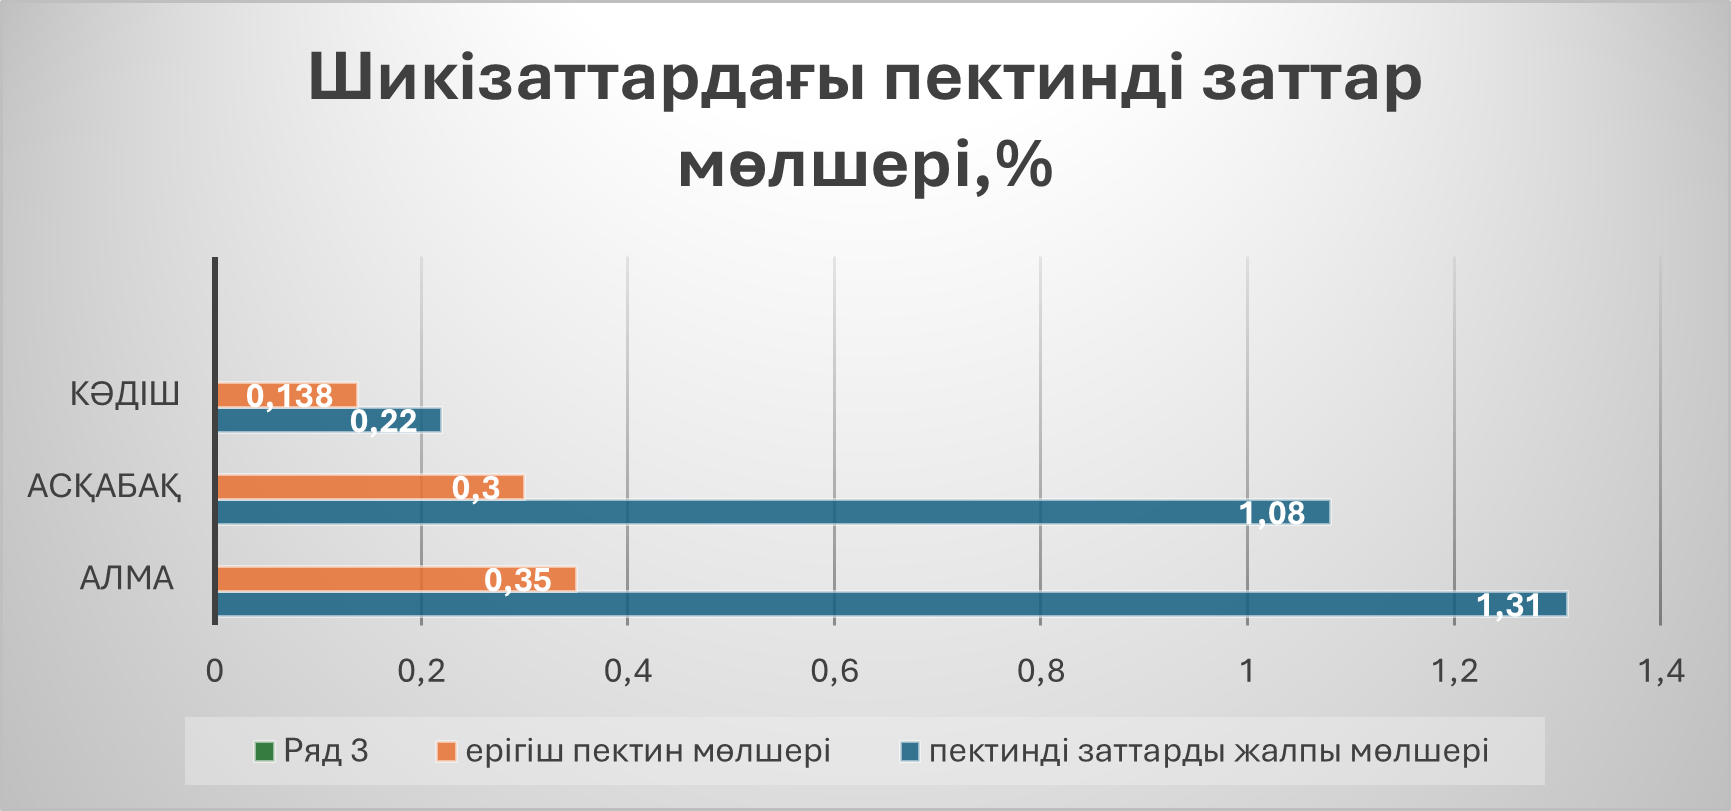
\includegraphics[width=0.8\textwidth]{media/pish4/image9}
	\caption*{1 - сурет. Өсімдік шикізаттарындағы пектинді зат мөлшері}
\end{figure}

\begin{multicols}{2}
Алма, асқабақ және кәдіштен алынған пектин экстракттарының
антиоксиданттық белсенділігі «Цвет Яуза-01-АА» хроматография құрылғысы
арқылы зерттелді.

Пектин экстракттарының антиоксиданттық белсенділігі де үлгілер арасында
айырмашылық көрсетеді. Ең жоғары антиоксидант мөлшері алма экстрактында
анықталды - 1,243 мг/100 г, бұл асқабақтың көрсеткішінен сәл жоғары -
1,102 мг/100 г. Ал кәдіш айтарлықтай төмен антиоксиданттық белсенділікке
ие - 0,570 мг/100 г {[}12{]}.
\end{multicols}

\tcap{5 - кесте. Пектин экстракттарының антиоксиданттық белсенділігі}
\begin{longtblr}[
  label = none,
  entry = none,
]{
  width = \linewidth,
  colspec = {Q[465]Q[150]Q[148]Q[177]},
  cells = {c},
  cell{2}{4} = {r=3}{},
  vlines,
  hline{1-2,5} = {-}{},
  hline{3-4} = {1-3}{},
}
Көрсеткіштің атауы & Өлшем бірлігі & Нәтиже & Өлшеу аспабы\\
Алма экстрактындағы антиоксидант мөлшері & мг/100 г & 1,243±0,019 & Цвет Яуза-01-АА \\
Асқабақ экстрактындағы антиоксидант мөлшері & мг/100 г & 1,102±0,017 & \\
Кәдіш экстрактындағы антиоксидант мөлшері & мг/100 г & 0,57±0,0068 & 
\end{longtblr}

\begin{multicols}{2}
{\bfseries Қорытынды.} Осылайша, алма мен асқабақ пектиндік және
антиоксиданттық қасиеттері жағынан кәдішке қарағанда анағұрлым айқын
ерекшеленеді. Бұл алма мен асқабақты жоғары сапалы, айқын функционалдық
белсенділігі бар пектин экстракттарын алу үшін қолдануды ұсынуға
мүмкіндік береді {[}13,14{]}.

Ғылыми жұмыс барысында көкөніс дәмтағам консервілерін дайындауда фарштың
құрамына қосылатын күріштің орнын булгур және қарақұмық жармаларымен
алмастыру арқылы дәмтағам консервілерінің жаңа рецептуралары алынған.
Сондай-ақ жаңа жарма қосылған көкөніс дәмтағам консервілерінің
рецептураларын құрастыруда пектиндік және антиоксиданттық қасиеттері
жағынан ерекшеленетін алма және асқабақ пектиндерінің экстрактылары
қолданылды (кесте 6).
\end{multicols}

\tcap{5 - кесте. Булгур және қарақұмық жармалары және пектин экстрактылары қосылған көкөніс дәмтағам консервілерінің рецептуралары, \%}
\begin{longtblr}[
  label = none,
  entry = none,
]{
  cells = {c},
  cell{1}{1} = {r=2}{},
  cell{1}{2} = {c=2}{},
  cell{1}{4} = {c=2}{},
  vlines,
  hline{1,3-20} = {-}{},
  hline{2} = {2-5}{},
}
Шикізаттар мен қосымша  материалдар атауы & Булгур &  & Қарақұмық & \\
 & 1 & 2 & 1 & 2\\
Тәтті бұрыш & 20 & 20 & 20 & 20\\
Пассерленген пияз & 7 & 7 & 7 & 7\\
Пассерленген сәбіз & 13 & 13 & 13 & 13\\
Пассерленген ақ тамырлар & 6 & 6 & 6 & 6\\
Пассерленген сарымсақ & 1,5 & 1,5 & 1,5 & 1,5\\
Аскөк & 0,5 & 0,5 & 0,5 & 0,5\\
Қызанақ езбесі, 12 \% & 12 & 12 & 12 & 12\\
Сұйық май & 14 & 14 & 14 & 14\\
Ұн & 2 & 2 & 2 & 2\\
Тұз & 3 & 3 & 3 & 3\\
Қант & 3 & 3 & 3 & 3\\
Қара бұрыш & 0,5 & 0,5 & 0,5 & 0,5\\
Хош иісті бұрыш & 0,5 & 0,5 & 0,5 & 0,5\\
Буланған қарақұмық & - & - & 15 & 15\\
Буланған булгур & 15 & 15 & - & -\\
Алма пектинінің экстрактысы & 2 & & 2 & \\
Асқабақ пектинінің экстрактысы & & 2 & & 2
\end{longtblr}

\begin{multicols}{2}
Осы рецептуралар бойынша алынған көкөніс дәмтағам консервілері
органолептикалық көрсеткіштері, яғни сыртқы түрі, дәмі, иісі бойынша өте
жоғары бағаға ие болды {[}15{]}.

\emph{{\bfseries Қаржыландыру.}Мақала БМҚ №BR24993031 «Табиғи
антиоксиданттар мен биологиялық белсенді заттармен байытылған күнделікті
рационға арналған пайдалы тағам өнімдерін дайындау технологиясын
әзірлеу» жобасының № 2-іс-шара тақырыбы «Белсенді пектинге бай экстракт
қосылған көкөніс консервілерінің (дәмтағам және түскі асқа арналған)
өндіру технологиясын әзірлеу» аясында жазылған.}
\end{multicols}

\begin{center}
{\bfseries Әдебиеттер}
\end{center}

\begin{references}
1. Блинова О.А., Праздничкова Н.В., Макушин А.Н., Троц А.П. Безопасность
и качество консервов на овощной основе для питания детей раннего
возраста // Материалы IХ Международной научно-практической конференции,
посвященной 20-летию специальности: «Технология и продукты здорового
питания»;Саратов. Саратов: ООО «Центр социальных агроинноваций СГАУ»,
2015. С.45--50.

2. Павловская, Л. М. Перспективные направления научных исследований
процессов консервирования овощей и фруктов: производство
ферментированных продуктов / Л. М. Павловская, С. Н. Голубева // Пищевая
промышленность: наука и технологии. -- 2017. -- №1(35). - С.63-68.

3. Киселева Т.Ф., Миллер Ю.Ю., Вечтомова Е.А. Технохимический контроль
производства овощных консервов . - Кемерово.: КемГУ, 2014.- 126 с. ISBN
978-5-89289-818-8

4. Манжесов В.И., Попов И.А., Щедрин Д.С., Калашникова С.В., Тертычная
Т.Н., Хабаров Н.Н., Курчаева Е.Е., Сысоева М.Г. Технология хранения,
переработки и стандартизация растениеводческой продукции. Учебник.-
СПб.: Троицкий мост, 2014.- 704 c. ISBN978-5-904406-07-3

5. Смотраева И.В., Баланов П.Е. Технология продуктов из растительного
сырья.- СПб.:НИУИТ, 2014.- 78 стр.

6. Сенгирбекова~Л.К., Сыздықова~Л.С. Определение качества овощных
закусочных консервов с различными крупами//Вестник Алматинского
технологического университета.- 2020.- № 3. - С.35-39.~
\href{https://doi.org/10.48184/2304-568X-2020-3-35-39}{DOI
10.48184/2304-568X-2020-3-35-39}

7. Ә.Ізтаев, К.Б.Байболов,А. Б.Мынбаева Жарма және жарма концентраттары
технологиясы, Алматы Технологиялық университеті, Алматы 2014.- 408 б.
ISBN 978-601-7427-49-8

8. Елисеева Л. Г. Товароведение и экспертиза продуктов переработки
плодов и овощей: Учебник для бакалавров / Л. Г. Елисеева, Т. Н. Иванова,
О. В. Евдокимова.-3-е изд. - М.: Издательско-торговая корпорация «Дашков
и К°», 2016.374 c. ISBN 978-5-394-02366-8

9. Романюк Т.И., Чусова А.Е., Новикова И.В. Методы исследования сырья и
продуктов растительного происхождения (теория и практика).-Воронежский
государственный университет инженерных технологий?2 014.- 160 c. ISBN
978-5-00032-075-4

10. Азимова С.Т. Обеспечение безопасности и детоксикационных свойств
продуктов питания на основе тыквенного пектина// диссертация на
соискание степени доктора философии (PhD), Алматы, 2018, 147 стр.

11. Лисовицкая Е. П., Патиева С. В., Родионова Л. Я., Шакота Ю.
Н. Пектин --- основной источник борьбы с вредными веществами /
Приоритетные направления развития пищевой индустрии. Матер. науч.-практ.
конф. - Ставрополь, 2016. С.385 -- 388.

12. Бухарова А. Р., Степанюк Н. В., Бухаров А. Ф.~Химический анализ
мякоти плодов тыквы крупноплодной на содержание низкомолекулярных
антиоксидантов / Вестн. Рос. гос. аграр. заоч. унив.- 2014. -№ 17.- С.
13 - 17.

13. Голубкина Н. А., Химич Г. А., Антошкина М. С. и др.~Особенности
каротиноидного состава тыквы «Конфетка», перспективы использования /
Овощи России. - 2021.- № 1. - С.111 - 116. DOI
10.18619/2072-9146-2021-1-111-116.

14. Shelenga T. V., Piskunova T. M., Malyshev L. L., et al.~Seed oil
biochemical composition of cultivated Cucurbita L. species from the VIR
collections grown in the Astrakhan province of the Russian Federation /
Agronomy.- 2020.- Vol.10(10). -P.1491.
\href{https://doi.org/10.3390/agronomy10101491}{DOI 10.3390/agronomy10101491}

15. Селиванова М.В., Романенко Е.С., Барабаш И.П., Есаулко Н.А., Сосюра
Е.А., Айсанов Т.С. Технология хранения и переработки плодов и овощей.
Учебный практикум. - Ставрополь: Ставропольский государственный аграрный
университет, Параграф, 2017.- 80 cтр.
\end{references}

\begin{center}
{\bfseries References}
\end{center}

\begin{references}
1. Blinova O.A., Prazdnichkova N.V., Makushin A.N., Troc A.P.
Bezopasnost'{} i kachestvo konservov na ovoshhnoj osnove
dlja pitanija detej rannego vozrasta // Materialy IH Mezhdunarodnoj
nauchno-praktiche\-skoj konferencii, posvjashhennoj 20-letiju
special' nosti: «Tehnologija i produkty zdorovogo
pitanija»; Saratov. Saratov: OOO «Centr social' nyh
agroinnovacij SGAU», 2015. S.45--50. {[}in Russian{]}

2. Pavlovskaja, L. M. Perspektivnye napravlenija nauchnyh issledovanij
processov konservirovanija ovosh\-hej i fruktov: proizvodstvo
fermentirovannyh produktov/L. M. Pavlovskaja, S. N. Golubeva //
Pishhevaja promyshlennost': nauka i tehnologii. - 2017. -
№1(35). - S.63-68. {[}in Russian{]}

3. Kiseleva T.F., Miller Ju.Ju., Vechtomova E.A. Tehnohimicheskij
kontrol'{} proizvodstva ovoshhnyh kon\-servov .- Kemerovo.:
KemGU, 2014.- 126 s. ISBN 978-5-89289-818-8.{[}in Russian{]}

4. Manzhesov V.I., Popov I.A., Shhedrin D.S., Kalashnikova S.V.,
Tertychnaja T.N., Habarov N.N., Kur\-chaeva E.E., Sysoeva M.G. Tehnologija
hranenija, pererabotki i standartizacija rastenievodcheskoj produk\-cii.
Uchebnik.- SPb.: Troickij most, 2014.- 704 c.
ISBN978-5-904406-07-3.{[}in Russian{]}

5. Smotraeva I.V., Balanov P.E. Tehnologija produktov iz
rastitel' nogo syr' ja.- SPb.:NIUIT,
2014. - 78 str. {[}in Russian{]}

6. Sengirbekova L.K., Syzdyқova L.S. Opredelenie kachestva ovoshhnyh
zakusochnyh konservov s razlich\-nymi krupami//Vestnik Almatinskogo
tehnologicheskogo universiteta.- 2020.- № 3. - S.35-39. DOI\\
10.48184/2304-568X-2020-3-35-39.{[}in Russian{]}

7. Ә.Іztaev, K.B.Bajbolov,A. B.Mynbaeva Zharma zhәne zharma
koncentrattary tehnologijasy, Almaty Tehnologijalyқ universitetі, Almaty
2014. - 408 b. ISBN 978-601-7427-49-8.{[}in Kazakh{]}

8. Eliseeva L. G. Tovarovedenie i jekspertiza produktov pererabotki
plodov i ovoshhej: Uchebnik dlja bakalavrov / L. G. Eliseeva, T. N.
Ivanova, O. V. Evdokimova.-3-e izd. - M.:
Izdatel' sko-torgovaja korpora\-cija «Dashkov i K°», 2016.
374 c. ISBN 978-5-394-02366-8.{[} in Russian{]}

9. Romanjuk T.I., Chusova A.E., Novikova I.V. Metody issledovanija
syr' ja i produktov rastitel' nogo
proishozhdenija (teorija i praktika).-Voronezhskij gosudarstvennyj
universitet inzhenernyh tehnologij?2 014.- 160 c. ISBN
978-5-00032-075-4.{[}in Russian{]}

10. Azimova C.T. Obecpechenie bezopacnocti i detokcikacionnyh cvojctv
produktov pitanija na ocnove tykvennogo pektina// diccertacija na
coickanie ctepeni doktora filocofii (PhD), Almaty, 2018.147 str.).
{[}in Russian{]}

11. Lisovickaja E. P., Patieva S. V., Rodionova L. Ja., Shakota Ju. N.
Pektin --- osnovnoj istochnik bor' by s vrednymi
veshhestvami / Prioritetnye napravlenija razvitija pishhevoj industrii.
Mater. nauch.-prakt. konf. - Stavropol', 2016. S.385 --
388. {[}in Russian{]}

12. Buharova A. R., Stepanjuk N. V., Buharov A. F. Himicheskij analiz
mjakoti plodov tykvy krupnoplod\-noj na soderzhanie nizkomolekuljarnyh
antioksidantov / Vestn. Ros. gos. agrar. zaoch. univ.- 2014. -№ 17.- S.
13 - 17. {[}in Russian{]}

13. Golubkina N. A., Himich G. A., Antoshkina M. S. i dr. Osobennosti
karotinoidnogo sostava tykvy «Konfetka», perspektivy
ispol' zovanija / Ovoshhi Rossii. - 2021.- № 1. - S.111
- 116. DOI 10.18619/2072-9146-2021-1-111-116.{[}in Russian{]}

14. Shelenga T. V., Piskunova T. M., Malyshev L. L., et al.~Seed oil
biochemical composition of cultivated Cucurbita L. species from the VIR
collections grown in the Astrakhan province of the Russian
Federation / Agronomy .-2020.- Vol.10(10). -P.1491.
\href{https://doi.org/10.3390/agronomy10101491}{DOI
10.3390/agronomy10101491}

15. Selivanova M.V., Romanenko E.S., Barabash I.P., Esaulko N.A.,
Sosjura E.A., Ajsanov T.S. Tehnolog\-ija hranenija i pererabotki plodov i
ovoshhej. Uchebnyj praktikum. - Stavropol':
Stavropol' skij gosudarstv\-ennyj agrarnyj universitet,
Paragraf, 2017.- 80 ctr. {[}in Russian{]}
\end{references}

\begin{authorinfo}
\emph{{\bfseries Авторлар туралы мәліметтер}}  

Сыздыкова Л.С. – т.ғ.к., ассоцирленген профессор, Алматы технологиялық
университеті АҚ, Алматы, Қазақстан, e-mail: laila.ss@mail.ru

Абдиева К.М. – б.ғ.к., Қазақстан Республикасы Ұлттық Биотехнология
орталығы, Астана, Қазақстан, e-mail: \\k.abdiyeva08@gmail.com

Шамбулова Г.Д. – т.ғ.к., Алматы технологиялық университеті, Алматы,
Қазақстан, e-mail: dosanbekgulnara@mail.ru

Азимова С. – PhD докторы, Алматы технологиялық университеті, Алматы,
Қазақстан, e-mail: sanaazimova@mail.ru

Жаксылыкова Г.Н. – т.ғ.к., Алматы технологиялық университеті, Алматы,
Қазақстан, e-mail: gulshatzh@mail.ru

Таева А.М. – т.ғ.д., профессор, Алматы технологиялық университеті,
Алматы, Қазақстан, e-mail: aigul\_taeva@mail.ru

\emph{{\bfseries Information about authors}}  

Syzdykova L. – Candidate of Technical Sciences, Associate Professor,
Almaty Technological University, Almaty, Kazakhstan, e-mail:
laila.ss@mail.ru

Abdiyeva K. – Candidate of Biological Sciences, National Center for
Biotechnology of the Republic of Kazakhstan, Astana, Kazakhstan,
e-mail: k.abdiyeva08@gmail.com

Shambulova G.D. – Candidate of Technical Sciences, Almaty
Technological University, Almaty, Kazakhstan, e-mail:\\
dosanbekgulnara@mail.ru

Azimova S. – PhD, Associate Professor, Almaty Technological
University, Almaty, Kazakhstan, e-mail: sanaazimova@mail.ru

Zhaksylikova G.N. – Candidate of Technical Sciences, Almaty
Technological University, Almaty, Kazakhstan, e-mail:\\
gulshatzh@mail.ru

Tayeva A. – Doctor of Technical Sciences, Professor, Almaty
Technological University, Almaty, Kazakhstan, e-mail:\\
aigul\_taeva@mail.ru
\end{authorinfo}
